% 第 14 题图（四边形 ABCD ＋ 正方形 ADPQ，面面垂直示意）：按固定源内容流矢量层精确值复刻（1 pt → 0.03515 cm，与全库同制）。
% 原点取 A 的 x=527.1415 pt、底缘（F 标签下缘）y（顶向下）=636.8870 pt；y 向上（Y = 636.8870 − y_页）。
% 源实测（figure-inventory §2）：3 条路径、9 条直线段，全实线、无虚线、无填充、无箭头，线宽 0.398。
%   正方形 ADPQ 按真形画出（轴对齐矩形，AD=102.0503、AQ=102.0463，差 0.0040 ⇒ 正方形）；
%   四边形 ABCD 按 45° 斜投影 + 1/2 缩短画成平行四边形（AB=51.0166 @ 44.997°、BC=102.0464、
%   CD=51.0138、DA=102.0503 —— AB/AD=0.49992≈1/2，与题干「ABCD 为正方形」自洽，属源内作图约定 S-2）。
%   E 为 AB 中点（源 p45 起点页 pt (545.1796,606.2505)，与中点解析值差 0.0019，本图照 p45 起点抄录）、
%   F 为 BC 中点（与 p44 末段终点逐位一致）、M 在 PQ 上、按源选定位置画在 Q→P 的 3/4 处
%   （归一化 0.749990 —— M 是动点，源取的代表位置非中点，照源保留，见 S-6）。
%   线段 9 条＝四边形 4（AB、BC、CD、DA，DA 为两面的公共棱）+ 正方形 3（DP、PQ、QA）+ AF + EM；
%   图中不画对角线，也无 EB/BF 之外的辅助线。标签 9 个（A、B、C、D、E、F、M、P、Q），照源字形盒中心定位。
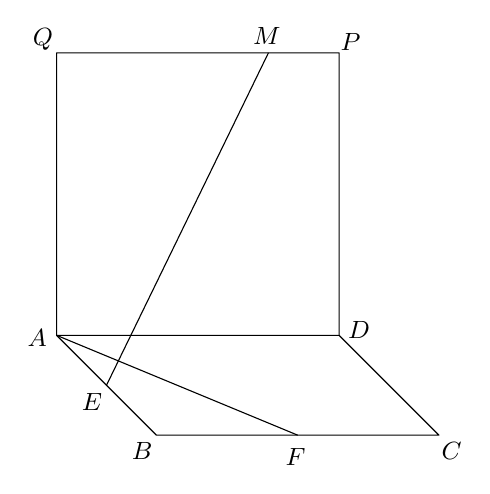
\begin{tikzpicture}[x=0.03515cm,y=0.03515cm,every node/.style={font=\small,inner sep=0pt},
  gl/.style={line width=0.398bp,line join=round}]
% ===== p43：四边形 ABCD（AB–BC–CD–DA；DA 为四边形与正方形的公共棱）=====
\draw[gl] (0,48.6707)--(36.0761,12.5985)--(138.1225,12.5985)--(102.0503,48.6707)--cycle;
% ===== p44：正方形 ADPQ（DP–PQ–QA）＋ 线段 AF（F 为 BC 中点）=====
\draw[gl] (102.0503,48.6707)--(102.0503,150.7170)--(0,150.7170)--(0,48.6707)--(87.0993,12.5985);
% ===== p45：线段 EM（E 为 AB 中点，M 在 PQ 的 Q→P 3/4 处）=====
\draw[gl] (18.0381,30.6365)--(76.5367,150.7170);
% ===== 标签 9 个（照源字形盒中心定位）=====
\node at (-4.9310,155.7090) {\(Q\)};
\node at (75.9635,156.7310) {\(M\)};
\node at (106.2500,154.6880) {\(P\)};
\node at (109.2650,50.7590) {\(D\)};
\node at (-6.9730,47.7090) {\(A\)};
\node at (12.8030,24.7410) {\(E\)};
\node at (30.8795,6.7040) {\(B\)};
\node at (86.3690,4.6620) {\(F\)};
\node at (142.6775,6.7040) {\(C\)};
\end{tikzpicture}
